\pdfminorversion=4
\documentclass[aspectratio=169]{beamer}

\mode<presentation>
{
  \usetheme{default}
  \usecolortheme{default}
  \usefonttheme{default}
  \setbeamertemplate{navigation symbols}{}
  \setbeamertemplate{caption}[numbered]
  \setbeamertemplate{footline}[frame number]  % or "page number"
  \setbeamercolor{frametitle}{fg=white}
  \setbeamercolor{footline}{fg=black}
} 

\usepackage[english]{babel}
\usepackage[utf8x]{inputenc}
\usepackage{tikz}
\usepackage{courier}
\usepackage{array}
\usepackage{bold-extra}
\usepackage{minted}
\usepackage[thicklines]{cancel}
\usepackage{fancyvrb}

\xdefinecolor{dianablue}{rgb}{0.18,0.24,0.31}
\xdefinecolor{darkblue}{rgb}{0.1,0.1,0.7}
\xdefinecolor{darkgreen}{rgb}{0,0.5,0}
\xdefinecolor{darkgrey}{rgb}{0.35,0.35,0.35}
\xdefinecolor{darkorange}{rgb}{0.8,0.5,0}
\xdefinecolor{darkred}{rgb}{0.7,0,0}
\definecolor{darkgreen}{rgb}{0,0.6,0}
\definecolor{mauve}{rgb}{0.58,0,0.82}

\title[2019-10-03-yana-david]{Conversation with Yana and David about Awkward 1.0}
\author{Jim Pivarski}
\institute{Princeton University -- IRIS-HEP}
\date{October 3, 2019}

\usetikzlibrary{shapes.callouts}

\begin{document}

\logo{\pgfputat{\pgfxy(0.11, 7.4)}{\pgfbox[right,base]{\tikz{\filldraw[fill=dianablue, draw=none] (0 cm, 0 cm) rectangle (50 cm, 1 cm);}\mbox{\hspace{-8 cm}
\includegraphics[height=1 cm]{princeton-logo-long.png}\hspace{0.1 cm}\raisebox{0.1 cm}{
\includegraphics[height=0.8 cm]{iris-hep-logo-long.png}}\hspace{0.1 cm}}}}}

\begin{frame}
  \titlepage
\end{frame}

\logo{\pgfputat{\pgfxy(0.11, 7.4)}{\pgfbox[right,base]{\tikz{\filldraw[fill=dianablue, draw=none] (0 cm, 0 cm) rectangle (50 cm, 1 cm);}\mbox{\hspace{-8 cm}
\includegraphics[height=1 cm]{princeton-logo.png}\hspace{0.1 cm}\raisebox{0.1 cm}{
\includegraphics[height=0.8 cm]{iris-hep-logo.png}}\hspace{0.1 cm}}}}}

% Uncomment these lines for an automatically generated outline.
%\begin{frame}{Outline}
%  \tableofcontents
%\end{frame}

% START START START START START START START START START START START START START

\begin{frame}{Context: columnar data analysis}
\large
\vspace{0.5 cm}
\begin{columns}
\column{1.1\linewidth}
\begin{itemize}\setlength{\itemsep}{1 cm}
\item \textcolor{darkblue}{\Large uproot}: reads columnar data (``split'' in ROOT terminology) from ROOT files without reconstructing objects---leaving them as arrays or jagged arrays.

\vspace{0.25 cm}
\textcolor{gray}{\normalsize (used by CMS, ATLAS, LHCb, NOvA, nuclear physics, theory, and gamma-ray astronomy)}

\item \textcolor{darkblue}{\Large awkward-array}: presents columnar data as though they were arrays of objects.

\vspace{0.25 cm}
\textcolor{gray}{\normalsize (used by 41 other projects on GitHub, including uproot and Coffea)}

\item \textcolor{darkblue}{\Large Coffea}: more fully featured data analysis package, developed by Fermilab physicists.

\vspace{0.25 cm}
\textcolor{gray}{\normalsize (used by at least 8 CMS analyses)}
\end{itemize}
\end{columns}
\end{frame}

\begin{frame}{Columnar data structures}
\vspace{0.2 cm}
\begin{center}
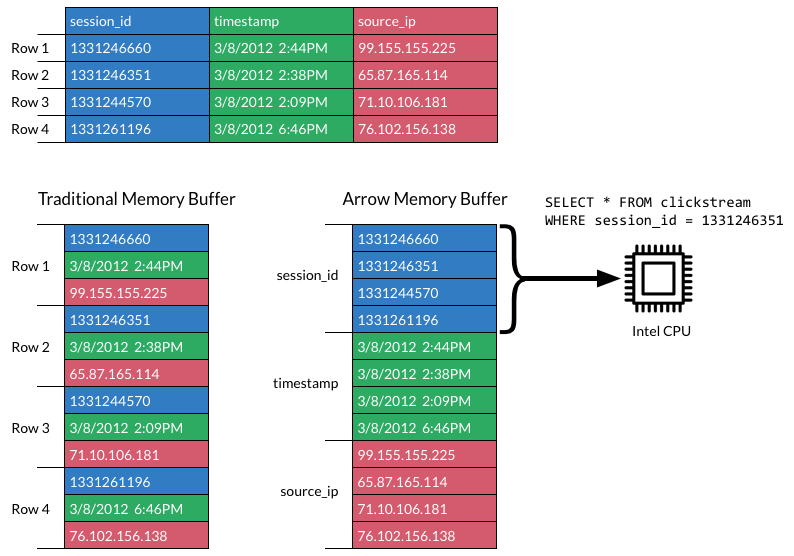
\includegraphics[width=0.7\linewidth]{simd.png}
\end{center}

Source: \textcolor{blue}{\url{http://arrow.apache.org}}
\end{frame}

\begin{frame}{Columnar data structures}
\begin{center}
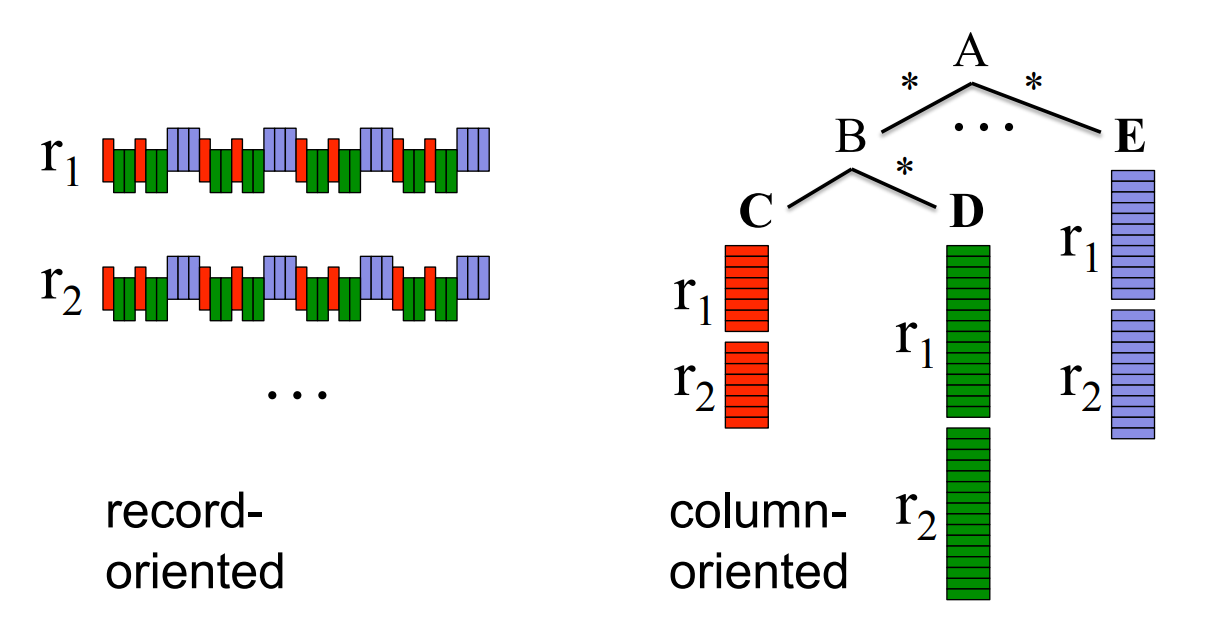
\includegraphics[width=0.95\linewidth]{google-dremel-fig1.png}
\end{center}

Source: \textcolor{blue}{\url{https://ai.google/research/pubs/pub36632}}
\end{frame}

\begin{frame}{On Scientific Linux, uproot/awkward is installed as often as Pandas}
\vspace{0.5 cm}
\begin{columns}
\column{1.2\linewidth}
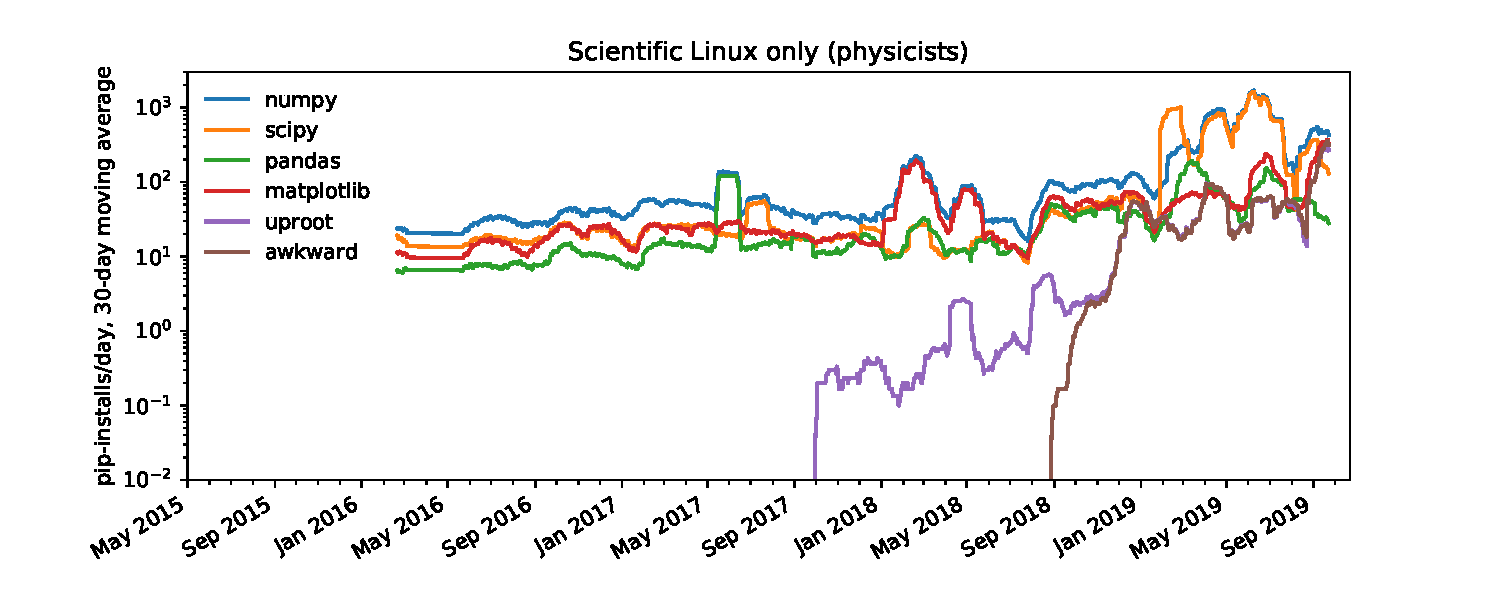
\includegraphics[width=\linewidth]{pip-scilinux-uproot.pdf}
\end{columns}
\end{frame}

\begin{frame}{And so is Coffea (very recently)\ldots}
\vspace{0.5 cm}
\begin{columns}
\column{1.2\linewidth}
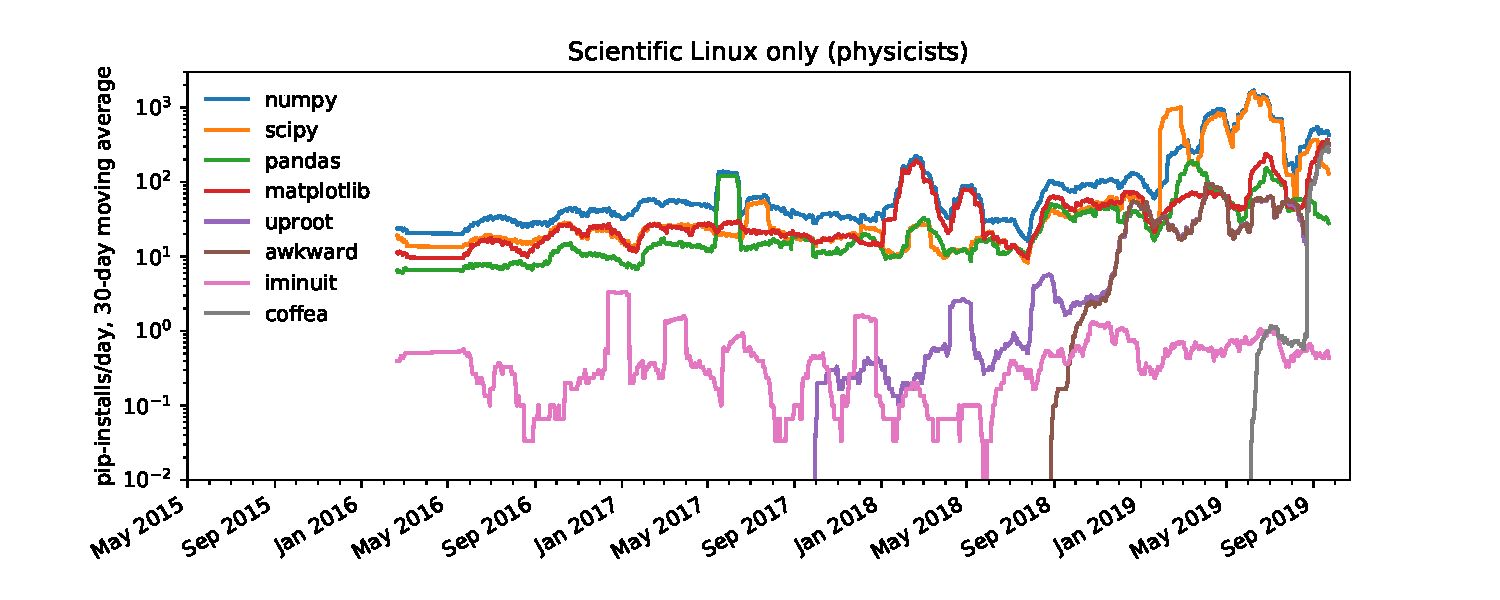
\includegraphics[width=\linewidth]{pip-scilinux-uproot-iminuit.pdf}
\end{columns}
\end{frame}

\begin{frame}{\ldots more so than deep learning libraries (TensorFlow and Torch)}
\vspace{0.5 cm}
\begin{columns}
\column{1.2\linewidth}
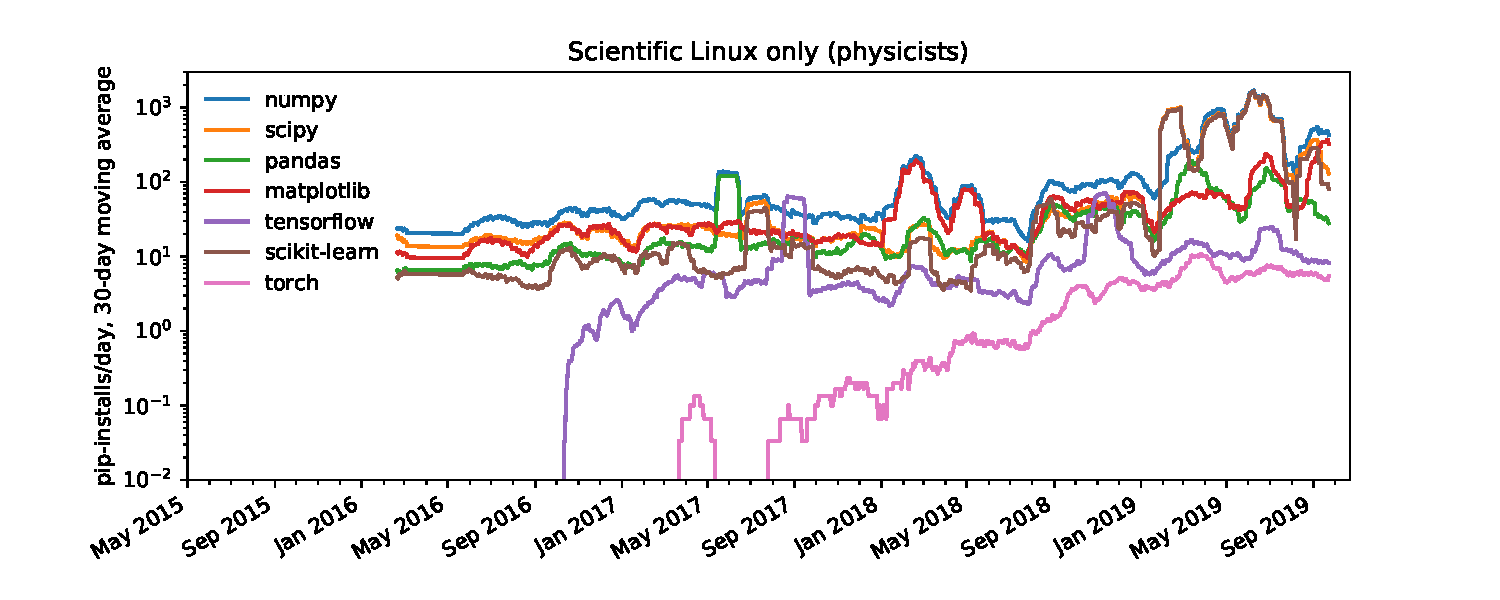
\includegraphics[width=\linewidth]{pip-scilinux-ml.pdf}
\end{columns}
\end{frame}

\begin{frame}{(Though in general, uproot is 4 orders of magnitude below Pandas)}
\vspace{0.5 cm}
\begin{columns}
\column{1.2\linewidth}
\only<1>{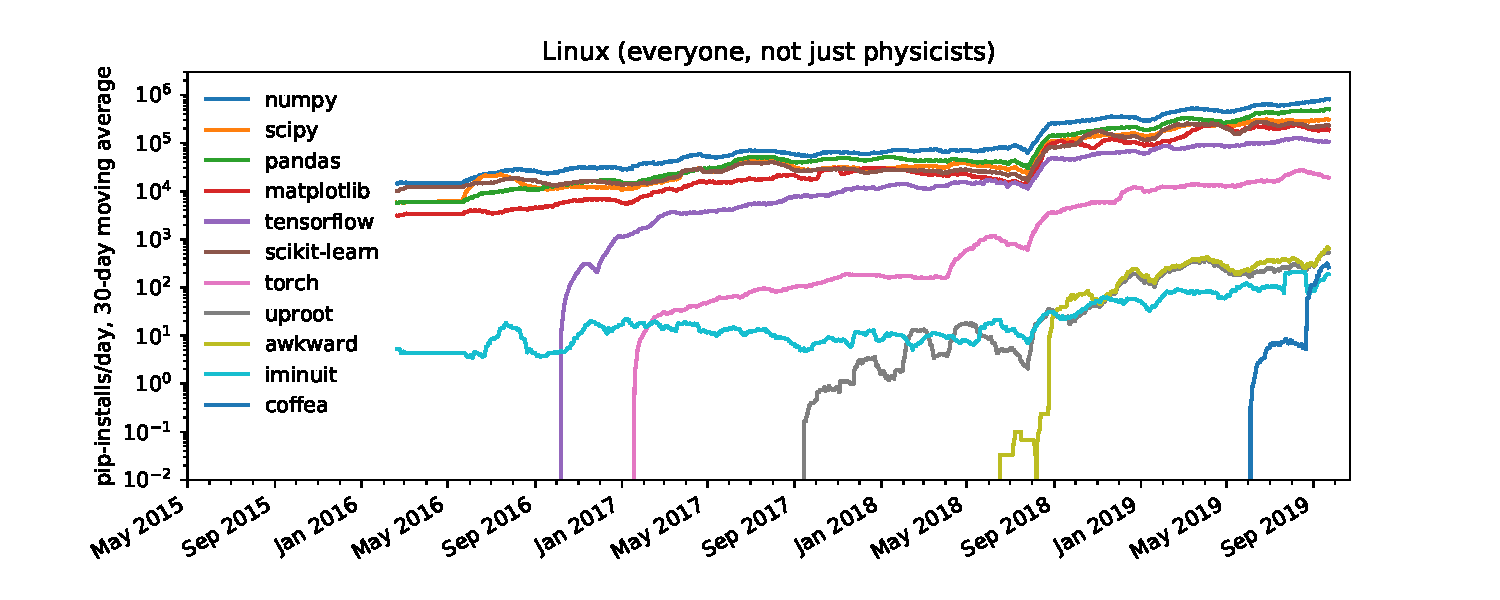
\includegraphics[width=\linewidth]{pip-linux.pdf}}\only<2>{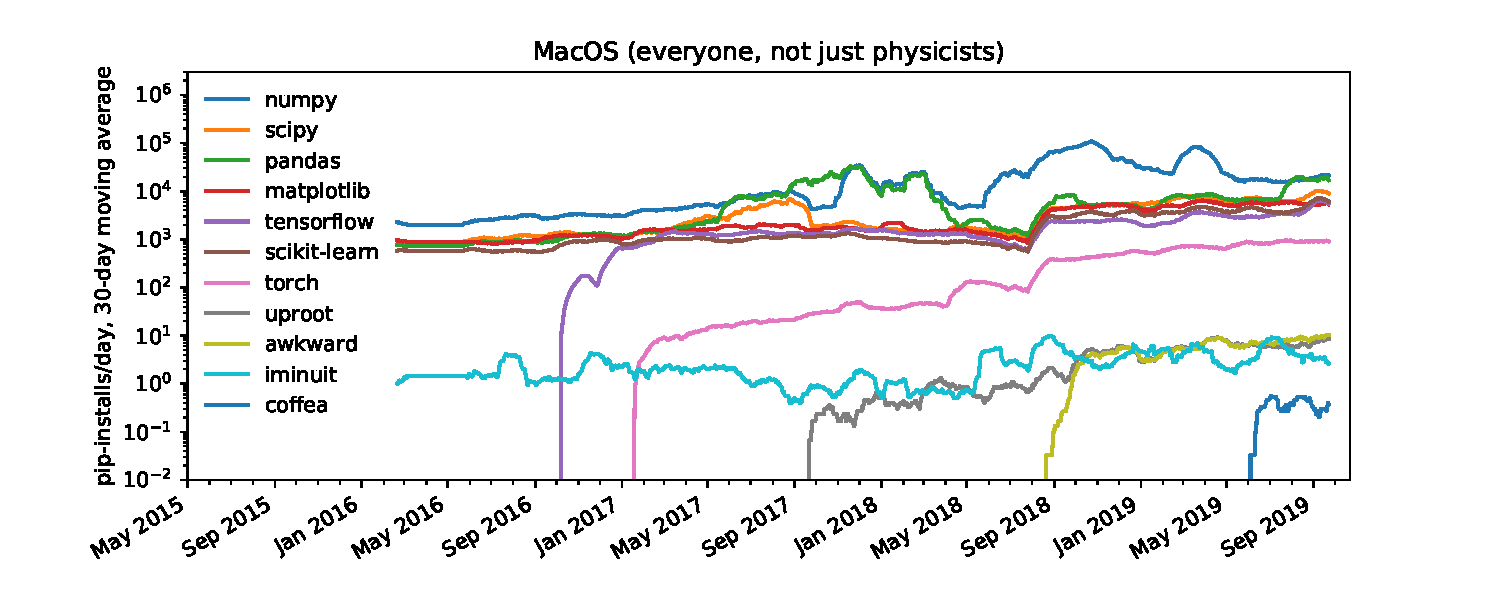
\includegraphics[width=\linewidth]{pip-macos.pdf}}\only<3>{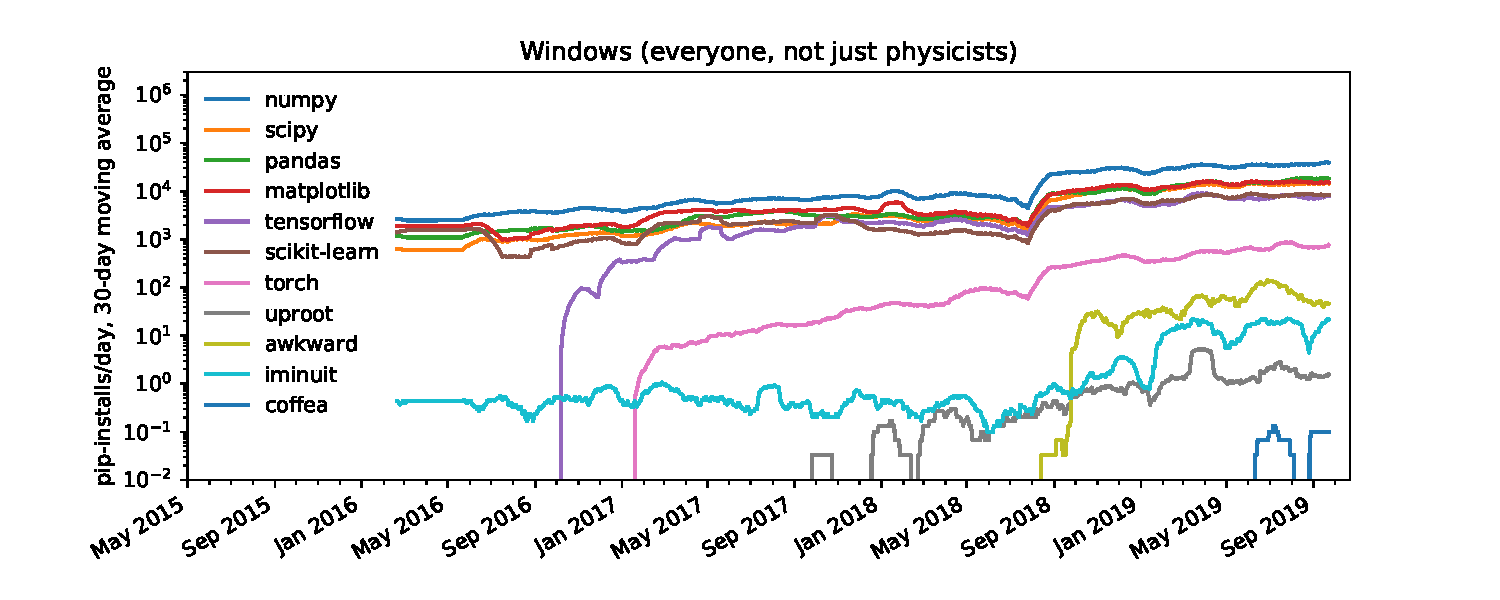
\includegraphics[width=\linewidth]{pip-windows.pdf}}
\end{columns}
\end{frame}

\begin{frame}{Uproot/Awkward maintainance is pretty much constant}
\Large
\vspace{0.75 cm}
\begin{columns}
\column{0.36\linewidth}
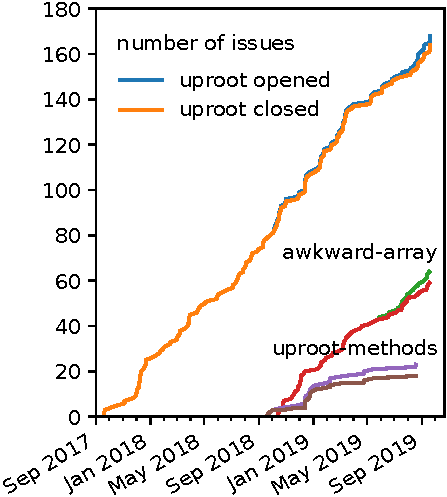
\includegraphics[width=\linewidth]{uproot-issues.pdf}

\column{0.72\linewidth}
\only<1>{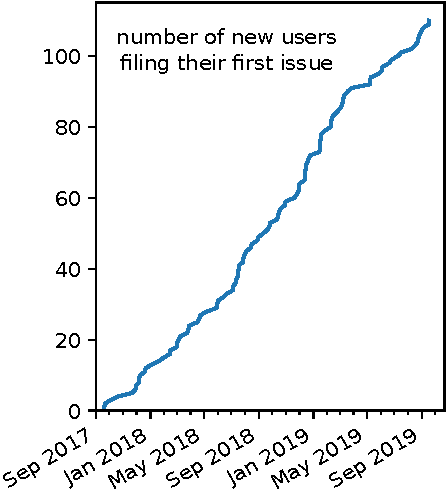
\includegraphics[width=0.5\linewidth]{uproot-users.pdf}\hfill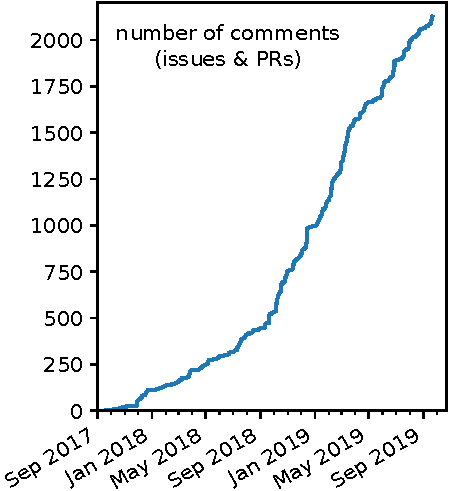
\includegraphics[width=0.5\linewidth]{uproot-comments.pdf}}\only<2->{\hfill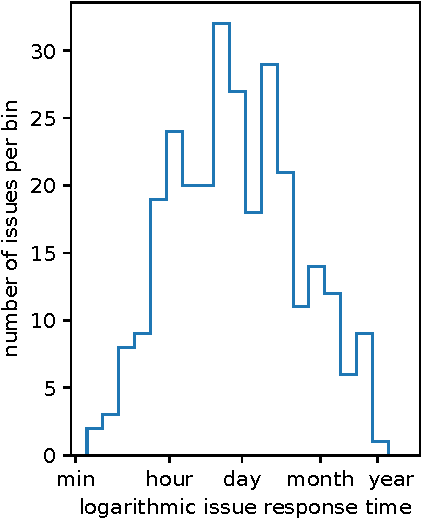
\includegraphics[width=0.45\linewidth]{uproot-response-time.pdf}\hfill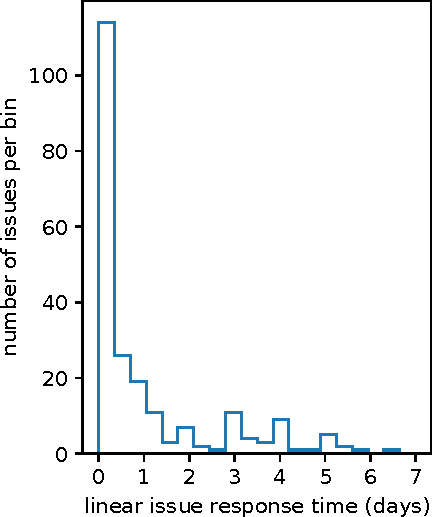
\includegraphics[width=0.45\linewidth]{uproot-response-time-linear.pdf}}
\end{columns}
\end{frame}

\begin{frame}{Awkward 1.0}
\large
\vspace{0.5 cm}
\begin{itemize}\setlength{\itemsep}{0.75 cm}
\item Uproot has been in use for 2 years now and is fine as-is. Maintenance with no major developments \textcolor{gray}{(apart from Pratyush's TTree-writing project)}.

\item Awkward has been in use for 1 year now, and there are

\vspace{0.2 cm}
\begin{itemize}\setlength{\itemsep}{0.2 cm}
\item \large structural issues: hard to keep interface consistent across all data types
\item \large interface issues: some visible features are confusing to users; need a semi-private between private and public.
\end{itemize}

\vspace{0.2 cm}
More detailed breakdown in this Google Doc (click): \normalsize

\vspace{0.2 cm}
\textcolor{blue}{\url{https://docs.google.com/document/d/1lj8ARTKV1_hqGTh0W_f01S6SsmpzZAXz9qqqWnEB3j4/edit?usp=sharing}}
\end{itemize}
\end{frame}

\begin{frame}{Awkward 1.0}
\vspace{0.2 cm}
\begin{columns}
\column{1.15\linewidth}
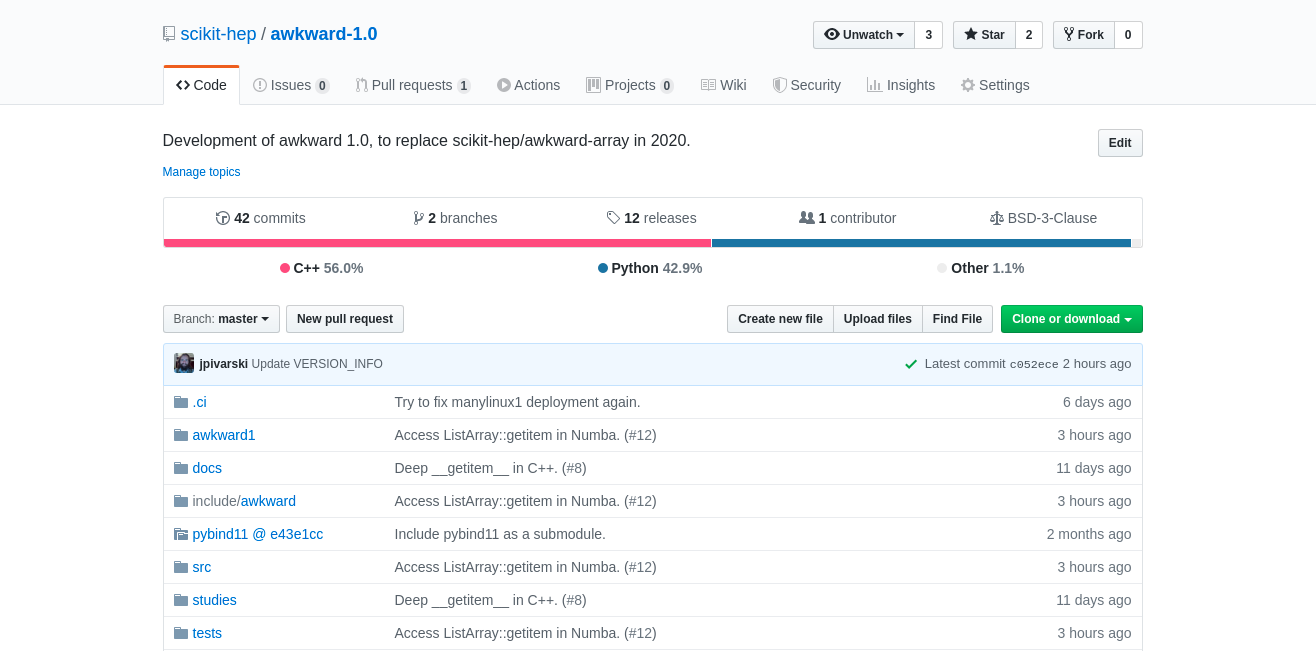
\includegraphics[width=\linewidth]{awkward-1-github.png}
\end{columns}
\end{frame}

\begin{frame}{Awkward 1.0}
\large
\vspace{0.5 cm}
\begin{columns}
\column{0.5\linewidth}
\vspace{-0.2 cm}

\textcolor{darkblue}{Layer 1:} Python user interface: a single \mintinline{python}{awkward.Array} class.
\vspace{\baselineskip}

\vspace{0.18 cm}
\textcolor{darkblue}{Layer 2:} Structure classes, ``layout''

(such as \mintinline{python}{JaggedArray}/\mintinline{python}{Table}).
\vspace{\baselineskip}

\vspace{0.18 cm}
\textcolor{darkblue}{Layer 3:} Memory management, array allocation and ownership; reference counting.
\vspace{\baselineskip}

\vspace{0.18 cm}
\textcolor{darkblue}{Layer 4:} Implementations, where we write \mintinline{python}{for} loops. The only layer that needs to be optimized.

\column{0.5\linewidth}
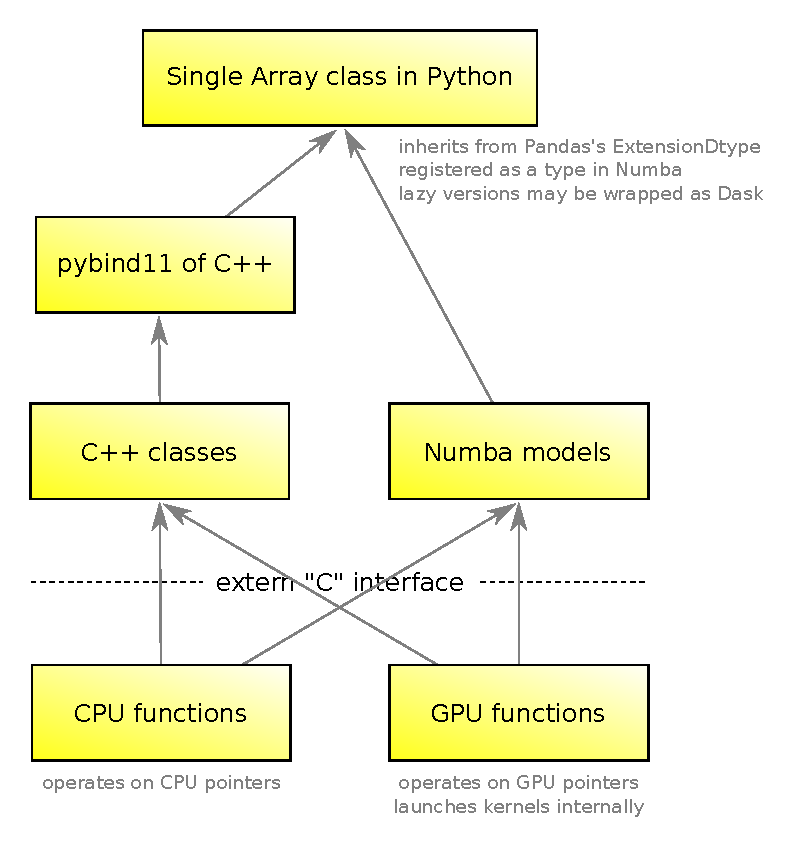
\includegraphics[width=\linewidth]{awkward-1-0-layers.pdf}
\end{columns}
\end{frame}

\begin{frame}[fragile]{Example of what layer 4 looks like}
\tiny
\vspace{0.05 cm}
\begin{columns}
\column{1.1\linewidth}
\begin{minted}{c++}
extern "C" {
  Error awkward_listarray32_getitem_next_at_64(int64_t* tocarry, const int32_t* fromstarts, const int32_t* fromstops,
                                               int64_t lenstarts, int64_t startsoffset, int64_t stopsoffset, int64_t at);
  Error awkward_listarray64_getitem_next_at_64(int64_t* tocarry, const int64_t* fromstarts, const int64_t* fromstops,
                                               int64_t lenstarts, int64_t startsoffset, int64_t stopsoffset, int64_t at);
}

template <typename C, typename T>
Error awkward_listarray_getitem_next_at(T* tocarry, const C* fromstarts, const C* fromstops, int64_t lenstarts,
                                        int64_t startsoffset, int64_t stopsoffset, int64_t at) {
  for (int64_t i = 0;  i < lenstarts;  i++) {
    int64_t length = fromstops[stopsoffset + i] - fromstarts[startsoffset + i];
    int64_t regular_at = at;
    if (regular_at < 0) {
      regular_at += length;
    }
    if (!(0 <= regular_at  &&  regular_at < length)) {
      return "index out of range";
    }
    tocarry[i] = fromstarts[startsoffset + i] + regular_at;
  }
  return kNoError;
}
Error awkward_listarray32_getitem_next_at_64(int64_t* tocarry, const int32_t* fromstarts, const int32_t* fromstops,
                                             int64_t lenstarts, int64_t startsoffset, int64_t stopsoffset, int64_t at) {
  return awkward_listarray_getitem_next_at<int32_t, int64_t>(tocarry, fromstarts, fromstops, lenstarts,
                                                             startsoffset, stopsoffset, at);
}
Error awkward_listarray64_getitem_next_at_64(int64_t* tocarry, const int64_t* fromstarts, const int64_t* fromstops,
                                             int64_t lenstarts, int64_t startsoffset, int64_t stopsoffset, int64_t at) {
  return awkward_listarray_getitem_next_at<int64_t, int64_t>(tocarry, fromstarts, fromstops, lenstarts,
                                                             startsoffset, stopsoffset, at);
}
\end{minted}
\end{columns}
\end{frame}

\begin{frame}[fragile]{Example of what layer 3 looks like (C++)}
\tiny
\vspace{0.05 cm}
\begin{columns}
\column{1.1\linewidth}
\begin{minted}{c++}
  template <>
  const std::shared_ptr<Content> ListArrayOf<int32_t>::getitem_next(const std::shared_ptr<SliceItem> head,
                                                                    const Slice& tail, const Index64& advanced) const {
    int64_t lenstarts = starts_.length();
    if (stops_.length() < lenstarts) {
      throw std::invalid_argument("len(stops) < len(starts)");
    }

    if (head.get() == nullptr) {
      return shallow_copy();
    }

    else if (SliceAt* at = dynamic_cast<SliceAt*>(head.get())) {
      assert(advanced.length() == 0);
      std::shared_ptr<SliceItem> nexthead = tail.head();
      Slice nexttail = tail.tail();
      Index64 nextcarry(lenstarts);
      Error err = awkward_listarray32_getitem_next_at_64(
        nextcarry.ptr().get(),
        starts_.ptr().get(),
        stops_.ptr().get(),
        lenstarts,
        starts_.offset(),
        stops_.offset(),
        at->at());
      std::shared_ptr<Content> nextcontent = content_.get()->carry(nextcarry);
      return nextcontent.get()->getitem_next(nexthead, nexttail, advanced);
    }

    else if (SliceRange* range = dynamic_cast<SliceRange*>(head.get())) {
      ...
\end{minted}
\end{columns}
\end{frame}

\begin{frame}[fragile]{Example of what layer 3 looks like (Numba)}
\tiny
\vspace{0.05 cm}
\begin{columns}
\column{1.1\linewidth}
\begin{minted}{python}
@numba.extending.register_model(ListOffsetArrayType)
class ListOffsetArrayModel(numba.datamodel.models.StructModel):
    def __init__(self, dmm, fe_type):
        members = [("offsets", fe_type.offsetstpe),
                   ("content", fe_type.contenttpe)]
        if fe_type.idtpe != numba.none:
            members.append(("id", fe_type.idtpe))
        super(ListOffsetArrayModel, self).__init__(dmm, fe_type, members)

@numba.extending.lower_builtin(operator.getitem, ListOffsetArrayType, numba.types.slice2_type)
def lower_getitem_slice(context, builder, sig, args):
    rettpe, (tpe, wheretpe) = sig.return_type, sig.args
    val, whereval = args

    proxyin = numba.cgutils.create_struct_proxy(tpe)(context, builder, value=val)

    proxyslicein = numba.cgutils.create_struct_proxy(wheretpe)(context, builder, value=whereval)
    proxysliceout = numba.cgutils.create_struct_proxy(numba.types.slice2_type)(context, builder)
    proxysliceout.start = proxyslicein.start
    proxysliceout.stop = builder.add(proxyslicein.stop, context.get_constant(numba.intp, 1))
    proxysliceout.step = context.get_constant(numba.intp, 1)

    proxyout = numba.cgutils.create_struct_proxy(tpe)(context, builder)
    proxyout.offsets = numba.targets.arrayobj.getitem_arraynd_intp(context, builder,
                                                                   tpe.offsetstpe(tpe.offsetstpe, numba.types.slice2_type),
                                                                   (proxyin.offsets, proxysliceout._getvalue()))
    proxyout.content = proxyin.content
    out = proxyout._getvalue()
    if context.enable_nrt:
        context.nrt.incref(builder, rettpe, out)
    return out
\end{minted}
\end{columns}
\end{frame}

\begin{frame}[fragile]{Example of what tests of layer 2 look like}
\tiny
\vspace{0.05 cm}
\begin{columns}
\column{1.1\linewidth}
\begin{minted}{python}
def test_listarray_slice_slice():
    assert awkward1.tolist(array1[2:]) == [[4.4, 5.5], [6.6], [7.7, 8.8, 9.9]]
    assert awkward1.tolist(array1[2:, 1:]) == [[5.5], [], [8.8, 9.9]]
    assert awkward1.tolist(array1[2:,:-1]) == [[4.4], [], [7.7, 8.8]]

def test_listarray_ellipsis():
    if not py27:
        assert awkward1.tolist(array1[Ellipsis, 1:]) == [[2.2, 3.3], [], [5.5], [], [8.8, 9.9]]
        assert awkward1.tolist(array2[Ellipsis, 1:]) == [[[2.2, 3.3], []], [[5.5]], [], [[], [8.8, 9.9]]]

def test_listarray_array_slice():
    assert awkward1.tolist(array2[[0, 0, 1, 1, 1, 0]]) == [[[1.1, 2.2, 3.3], []], [[1.1, 2.2, 3.3], []], [[4.4, 5.5]],
                                                           [[4.4, 5.5]], [[4.4, 5.5]], [[1.1, 2.2, 3.3], []]]
    assert awkward1.tolist(array2[[0, 0, 1, 1, 1, 0], :]) == [[[1.1, 2.2, 3.3], []], [[1.1, 2.2, 3.3], []], [[4.4, 5.5]],
                                                              [[4.4, 5.5]], [[4.4, 5.5]], [[1.1, 2.2, 3.3], []]]
    assert awkward1.tolist(array2[[0, 0, 1, 1, 1, 0], :, 1:]) == [[[2.2, 3.3], []], [[2.2, 3.3], []], [[5.5]], [[5.5]],
                                                                  [[5.5]], [[2.2, 3.3], []]]

def test_listarray_array():
    assert awkward1.tolist(array1[numpy.array([2, 0, 0, 1, -1])]) == [[4.4, 5.5], [1.1, 2.2, 3.3], [1.1, 2.2, 3.3], [],
                                                                      [7.7, 8.8, 9.9]]
    assert awkward1.tolist(array1[numpy.array([2, 0, 0, -1]), numpy.array([1, 1, 0, 0])]) == [5.5, 2.2, 1.1, 7.7]

    assert awkward1.tolist(array1_deep) == [[[0, 0], [1, 10], [2, 20]], [[3, 30], [4, 40], [5, 50]], [[6, 60], [7, 70],
                                                                                                      [8, 80]]]
    s = (numpy.array([2, 0, 0, -1]), numpy.array([1, 1, 0, 0]), numpy.array([0, 1, 0, 1]))
    assert (numpy.array([[[0, 0], [1, 10], [2, 20]], [[3, 30], [4, 40], [5, 50]], [[6, 60], [7, 70], [8, 80]]])[s].tolist()
              == awkward1.tolist(array1_deep[s]))

    s = (numpy.array([2, 0, 0, -1]), numpy.array([1, 1, 0, 0]), slice(1, None))
    assert (numpy.array([[[0, 0], [1, 10], [2, 20]], [[3, 30], [4, 40], [5, 50]], [[6, 60], [7, 70], [8, 80]]])[s].tolist()
              == awkward1.tolist(array1_deep[s]))
\end{minted}
\end{columns}
\end{frame}

\begin{frame}[fragile]{Usable in C++, too (for making interfaces to C++ libraries)}
\tiny
\vspace{0.05 cm}
\begin{columns}
\column{1.1\linewidth}
\begin{minted}{c++}
#include <cassert>

#include "awkward/Identity.h"
#include "awkward/RawArray.h"
#include "awkward/Slice.h"

using namespace awkward;

void slices() {
  RawArrayOf<float> data(Identity::none(), 9);
  *data.borrow(0) = 0.0f;
  *data.borrow(1) = 1.1f;
  *data.borrow(2) = 2.2f;
  *data.borrow(3) = 3.3f;
  *data.borrow(4) = 4.4f;
  *data.borrow(5) = 5.5f;
  *data.borrow(6) = 6.6f;
  *data.borrow(7) = 7.7f;
  *data.borrow(8) = 8.8f;
  *data.borrow(9) = 9.9f;

  Slice at1(std::vector<std::shared_ptr<SliceItem>>({ std::shared_ptr<SliceItem>(new SliceAt(1)) }), true);
  assert(*dynamic_cast<RawArrayOf<float>*>(data.getitem(at1).get())->borrow() == 1.1f);
  Slice at2(std::vector<std::shared_ptr<SliceItem>>({ std::shared_ptr<SliceItem>(new SliceAt(2)) }), true);
  assert(*dynamic_cast<RawArrayOf<float>*>(data.getitem(at2).get())->borrow() == 2.2f);

  Slice range1(std::vector<std::shared_ptr<SliceItem>>({ std::shared_ptr<SliceItem>(new SliceRange(1, 3, Slice::none())) }));
  assert(*dynamic_cast<RawArrayOf<float>*>(data.getitem(range1).get())->borrow(0) == 1.1f);

  Slice range2(std::vector<std::shared_ptr<SliceItem>>({ std::shared_ptr<SliceItem>(new SliceRange(Slice::none(), 4, 1)) }));
  assert(*dynamic_cast<RawArrayOf<float>*>(data.getitem(range2).get())->borrow(0) == 0.0f);
}
\end{minted}
\end{columns}
\end{frame}





\end{document}
